% !TEX TS-program = pdflatex
% !TEX encoding = UTF-8 Unicode

% This is a simple template for a LaTeX document using the "article" class.
% See "book", "report", "letter" for other types of document.

\documentclass[11pt]{article} % use larger type; default would be 10pt

\usepackage[utf8]{inputenc} % set input encoding (not needed with XeLaTeX)

%%% Examples of Article customizations
% These packages are optional, depending whether you want the features they provide.
% See the LaTeX Companion or other references for full information.

%%% PAGE DIMENSIONS
\usepackage{geometry} % to change the page dimensions
\geometry{a4paper} % or letterpaper (US) or a5paper or....
% \geometry{margin=2in} % for example, change the margins to 2 inches all round
% \geometry{landscape} % set up the page for landscape
%   read geometry.pdf for detailed page layout information

\usepackage{graphicx} % support the \includegraphics command and options

% \usepackage[parfill]{parskip} % Activate to begin paragraphs with an empty line rather than an indent

%%% PACKAGES
\usepackage{booktabs} % for much better looking tables
\usepackage{array} % for better arrays (eg matrices) in maths
\usepackage{paralist} % very flexible & customisable lists (eg. enumerate/itemize, etc.)
\usepackage{verbatim} % adds environment for commenting out blocks of text & for better verbatim
\usepackage{subfig} % make it possible to include more than one captioned figure/table in a single float
% These packages are all incorporated in the memoir class to one degree or another...

%%% HEADERS & FOOTERS
\usepackage{fancyhdr} % This should be set AFTER setting up the page geometry
\pagestyle{fancy} % options: empty , plain , fancy
\renewcommand{\headrulewidth}{0pt} % customise the layout...
\lhead{}\chead{}\rhead{}
\lfoot{}\cfoot{\thepage}\rfoot{}

%%% SECTION TITLE APPEARANCE
\usepackage{sectsty}
\allsectionsfont{\sffamily\mdseries\upshape} % (See the fntguide.pdf for font help)
% (This matches ConTeXt defaults)

%%% ToC (table of contents) APPEARANCE
\usepackage[nottoc,notlof,notlot]{tocbibind} % Put the bibliography in the ToC
\usepackage[titles,subfigure]{tocloft} % Alter the style of the Table of Contents
\renewcommand{\cftsecfont}{\rmfamily\mdseries\upshape}
\renewcommand{\cftsecpagefont}{\rmfamily\mdseries\upshape} % No bold!

%% Jason's article customizations:

\usepackage{amsmath}
\usepackage{units}
\usepackage{url}
\usepackage{hyperref}
\usepackage{listings}
\usepackage{float}
%%% END Article customizations

%%% The "real" document content comes below...

\title{Write-up for Problem Set 3 \\ of CMSC 733 }
\author{Jason Filippou}
%\date{} % Activate to display a given date or no date (if empty),
         % otherwise the current date is printed 

\begin{document}
\maketitle

\tableofcontents

\section{Expectation - Maximization for line fitting}

In this section, we analyze our implementation of the first part of the problem set.  

\subsection{Pure line fitting}
\label{sec:pureLineFit}
This is essentially the M-step of E-M, where all weights are 1. As such, it can be easily transformed to boil down to linear regression over a set of
2D variables. Specifically, let $\mathbf{D}$ be a 2 x n matrix of 2D data points, where the data points are in the columns:

$$\mathbf{D} = \begin{bmatrix} x_1 && x_2 && \dots && x_n \\ y_1 && y_2 && \dots && y_n \end {bmatrix}$$

This is the input to our method. Then, we can form the vector $\mathbf{y} = [y_1\ y_2\ \dots y_n]^T$ from the second row of $D$ and the 2 x n matrix $\mathbf{X}$ from the first row and a vector of all 1's:

$$\mathbf{X} = \begin{bmatrix} x_1 && x_2 && \dots && x_n \\ 1 && 1 && \dots && 1 \end {bmatrix}$$

In this form, the desired parameter vector $\hat{v} = [a\ b]^T$ is the solution to the following linear regression problem:

\begin{equation}
	\hat{v} = (X X^T) ^{-1}  Xy
\label{eqn:linreg}
\end{equation}

which, if properly unpacked, will convince the reader that it has exactly the same form as the one presented in Yair Weiss' notes.

Our results for the data provided are shown in figure \ref{fig:lineFitting}. As shown in figure \ref{fig:lineFitting}(c), for even simple, artificial datasets,
linear regression can often produce fits far away from the optimal fit (which cannot be linear, in this case).

\begin{figure}[H]
\centering
	\begin{tabular}{c c c}
		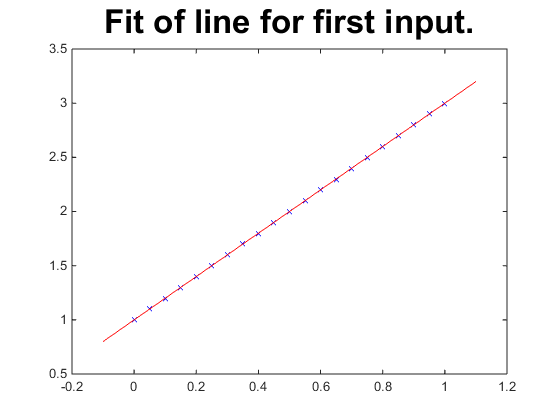
\includegraphics[width=.32\textwidth]{figures/inp1} &
		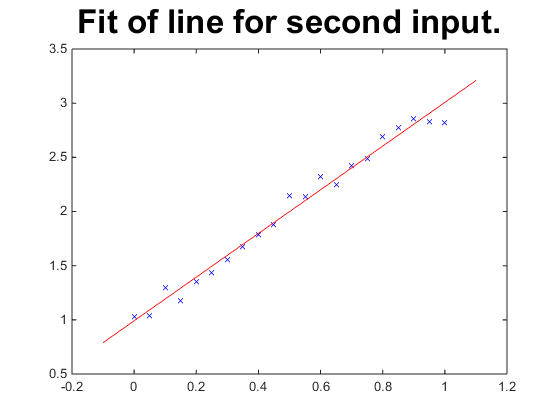
\includegraphics[width=.32\textwidth]{figures/inp2} &
		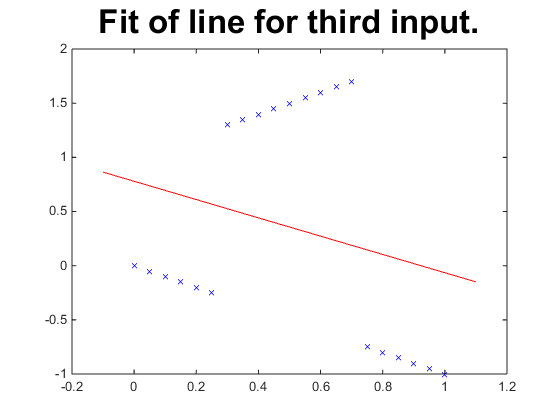
\includegraphics[width=.32\textwidth]{figures/inp3}   \\ 
		(a) & (b) & (c) 
	\end{tabular}
	\caption{Results for pure line fitting.}
	\label{fig:lineFitting}
\end{figure}

The code for this section can be found in the MATLAB function \texttt{fit\_line.m}. Note that, in that function, we transform the matrix $\textbf{X}$
such that the patterns are in the rows instead of the columns, and this changes equation \ref{eqn:linreg} to 

\begin{equation*}
	\hat{v} = (X^T X) ^{-1}  X^Ty
\end{equation*}
\subsection{Full E-M}

We now show how we can iteratively find a pair of good linear fits for a dataset of 2D points using the E-M algorithm, and examine certain cases where the algorithm has trouble finding good fits because of noisy data. We analyze the E and M steps in isolation and then we show our results when both steps are combined.

\subsubsection{`E' step}

In this step, the parameters of the lines $[a_1\ b_1]^T,\ [a_2\ b_2]^T$ are assumed to be known, and we estimate the $n$-dimensional weight vectors $\mathbf{w_1}$ and $\mathbf{w_2}$. We follow Yarr Weiss' notes on this. First, for $i \in \lbrace1, 2 \rbrace$, we compute the residual vectors:

\begin{equation}
	\mathbf{r_i} = a_i \cdot \mathbf{x} +  b_i - \mathbf{y} 
	\label{eqn:res}
\end{equation}

and then pass them through a softmin function to compute the relevant weight vectors:

\begin{equation}
	\mathbf{w_i} = \frac{e^{\nicefrac{-\mathbf{r_i}^2}{\sigma^2}}}{e^{\nicefrac{-\mathbf{r_1}^2}{\sigma^2}} + e^{\nicefrac{-\mathbf{r_2}^2}{\sigma^2}}}
	\label{eqn:softmin}
\end{equation}

The code for the E-step is available in the MATLAB function \texttt{Estep.m}.

\subsubsection{`M' step}

The `M' step consists of solving weighted linear least squares \footnote{\url{http://en.wikipedia.org/wiki/Least_squares\#Weighted_least_squares}}. The form of the problem is very similar to equation \ref{eqn:linreg}. If we form the n x n diagonal matrix $\mathbf{W}$ with the weights of every point along its main diagonal:

\[ W = 
\left(
 \begin{array}{ccccc}
   \tiny{w_1}\\
    & \tiny{w_2} & & \text{\large0}\\
    & & \dots\\
    & \text{\large0} & & \dots\\
    & & & & \tiny{w_n}
 \end{array}
\right)
\]

Then we would need to solve the equation:

\begin{equation}
	\hat{v} = (X W X^T) ^{-1}  WXy
	\label{eqn:wlsq}
\end{equation}

The code is available in the function file \texttt{Mstep.m}.

\subsubsection{Results}

In this section, we show our results on applying E-M in both the data used in section \ref{sec:pureLineFit} as well as data that has been altered by noise.

\begin{figure}[H]
	\centering
	\begin{tabular}{c c c}
		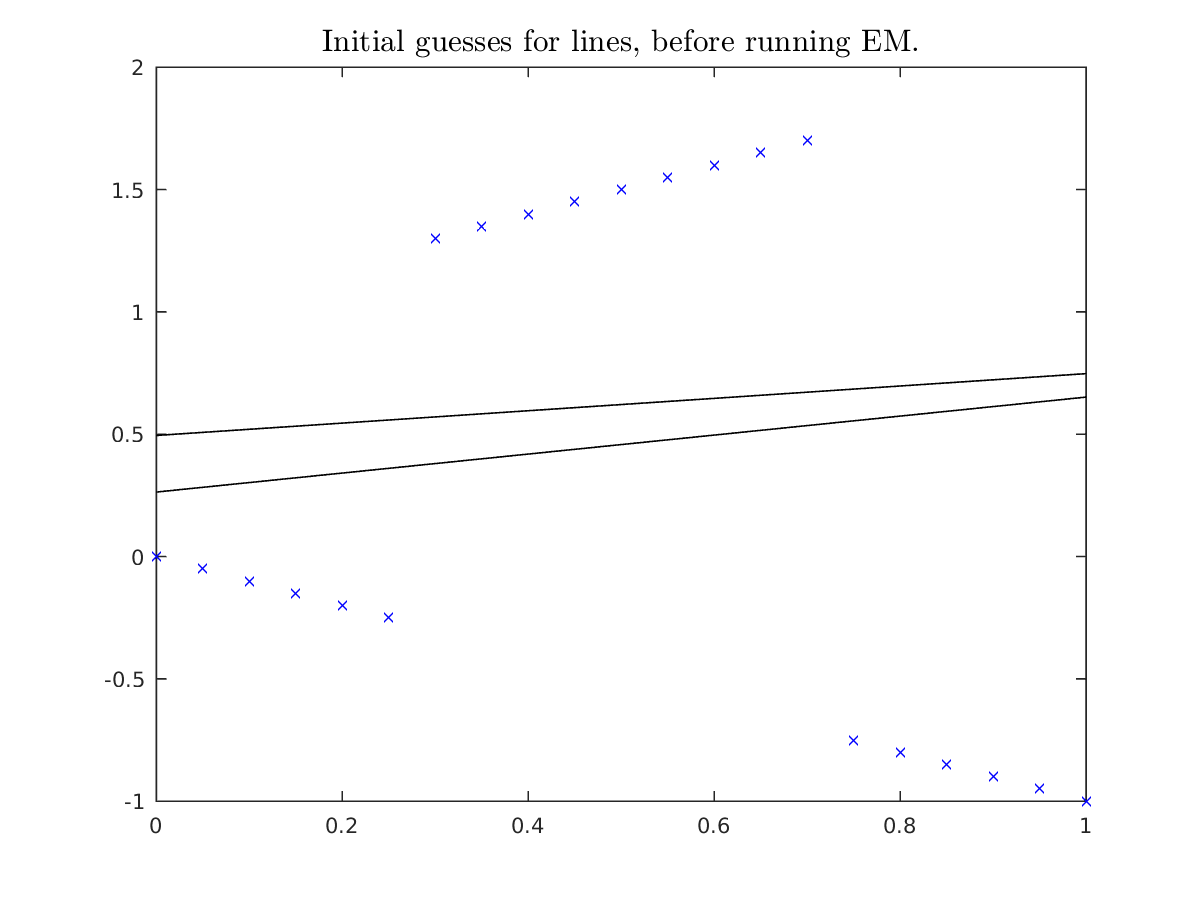
\includegraphics[scale=.35]{figures/beforeEM} & 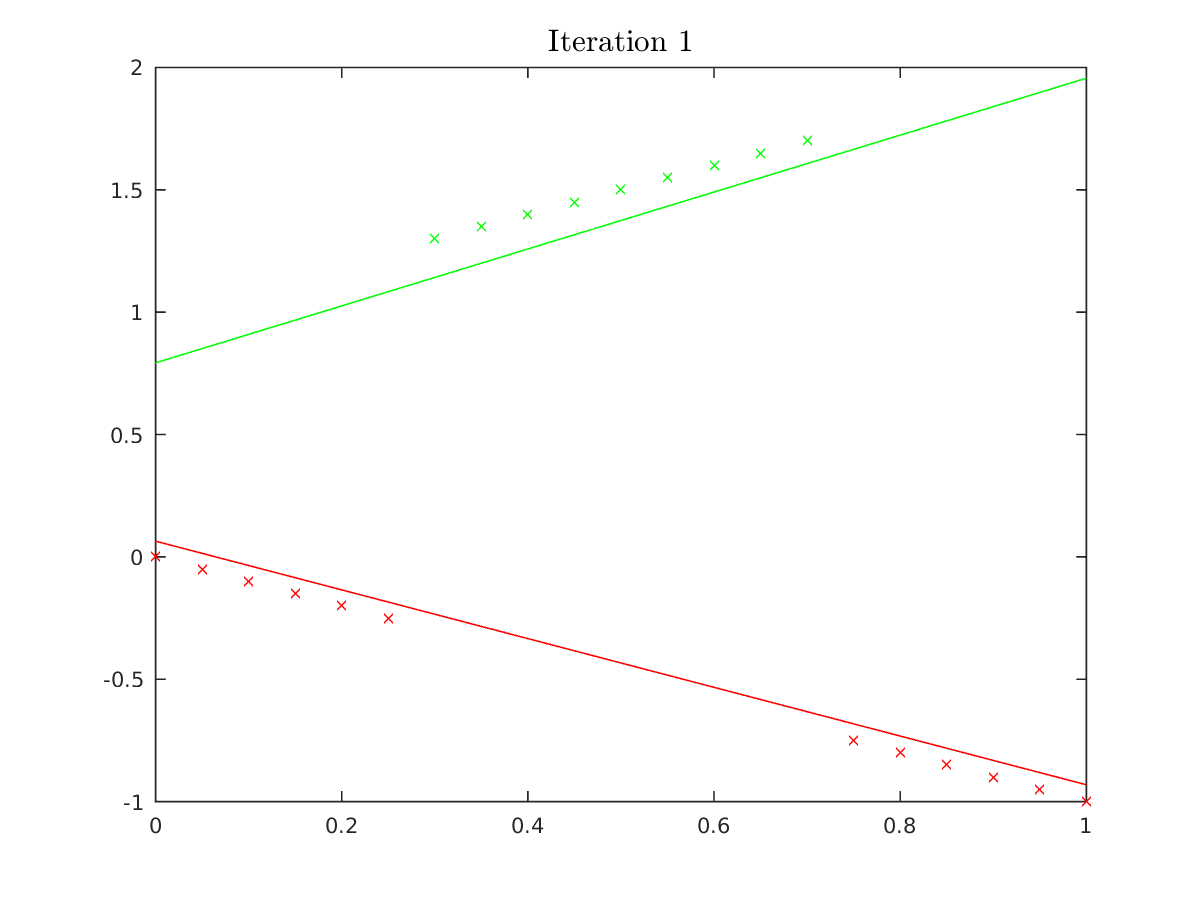
\includegraphics[scale=.35]{figures/iter1} \\
		(a) & (b) \\
		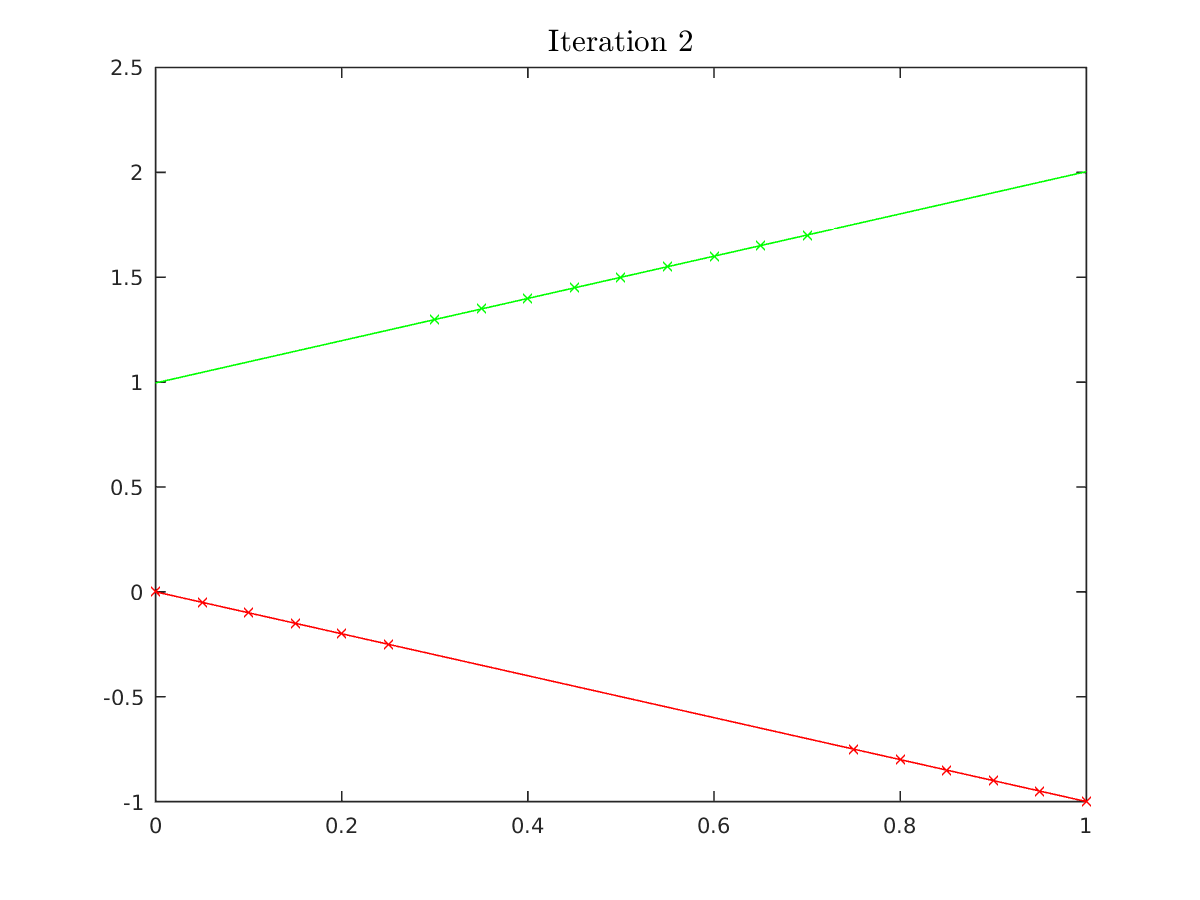
\includegraphics[scale=.35]{figures/iter2} & 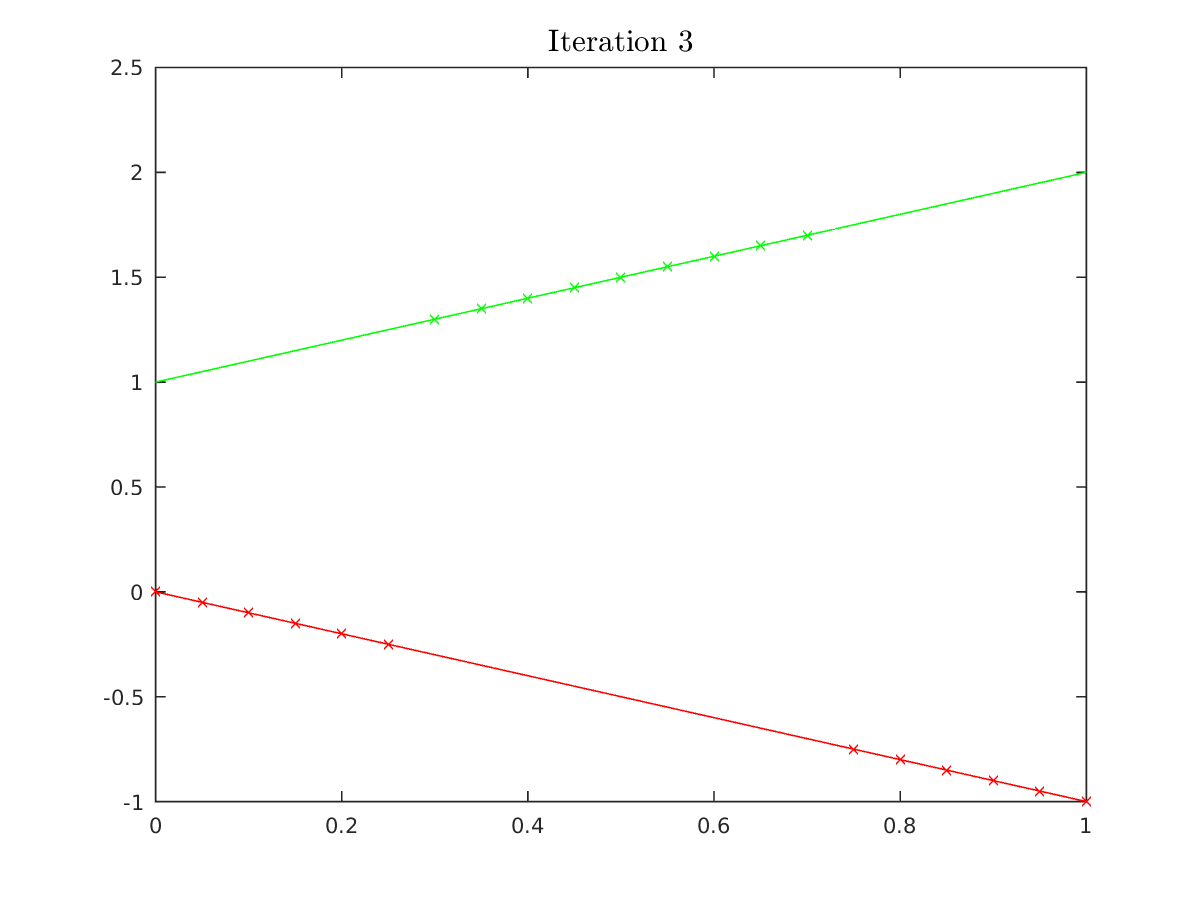
\includegraphics[scale=.35]{figures/iter3} \\ 
		(c) & (d) \\
		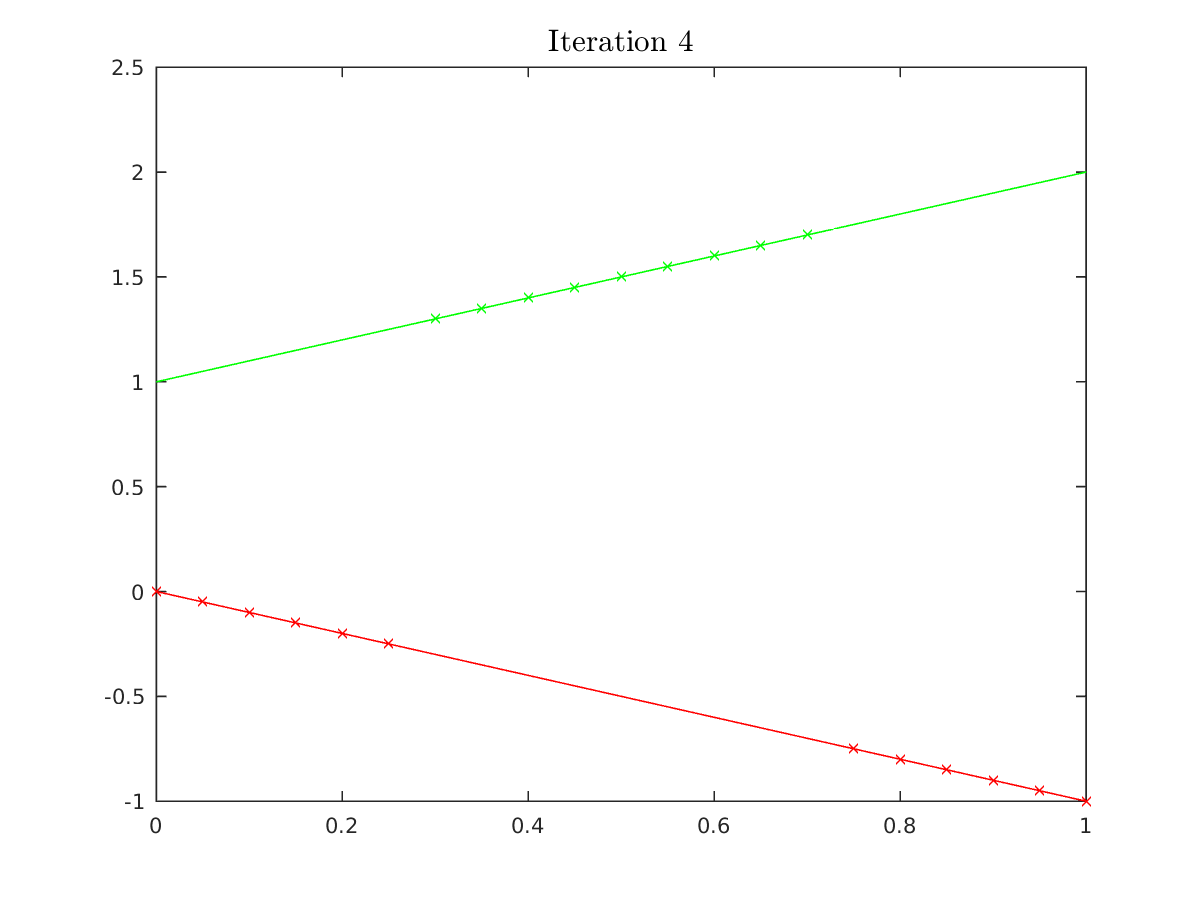
\includegraphics[scale=.35]{figures/iter4} & 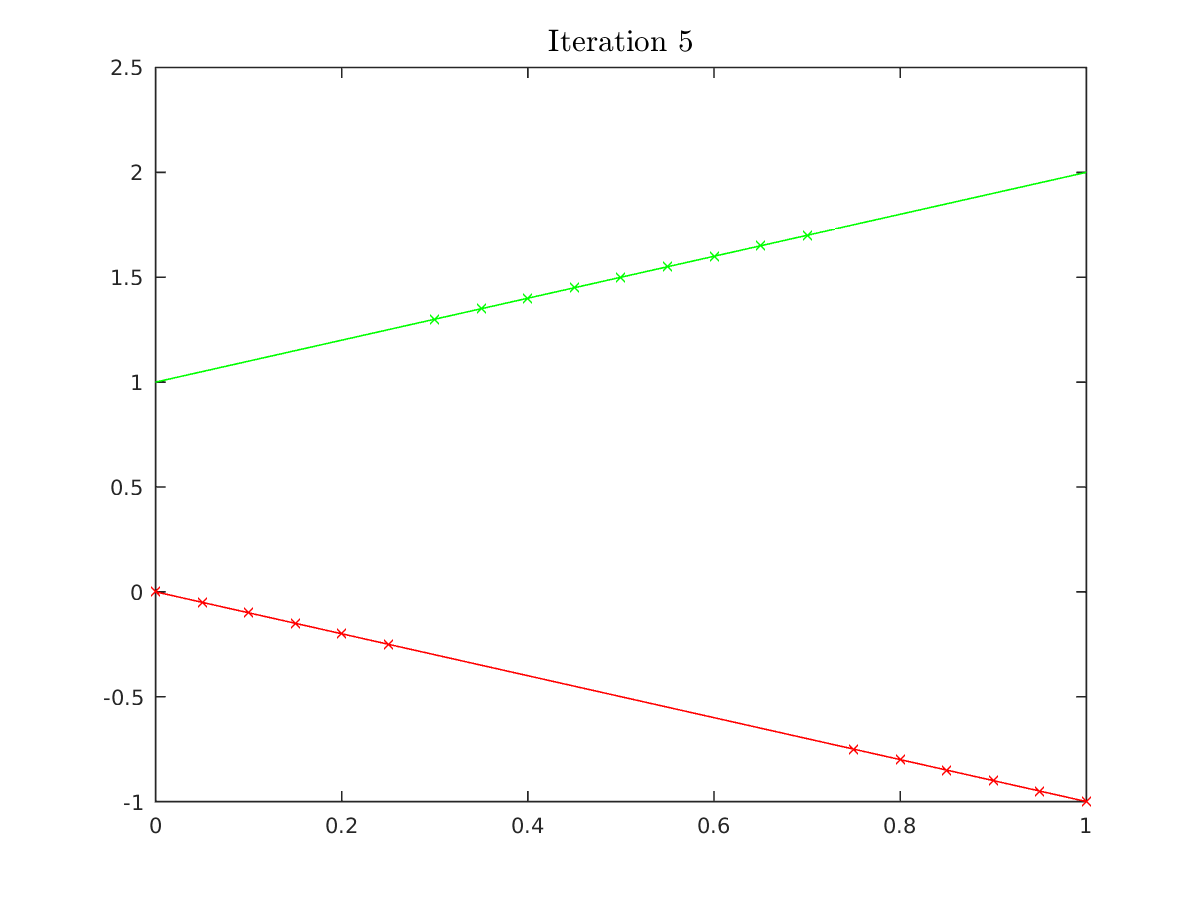
\includegraphics[scale=.35]{figures/iter5} \\ 				
		(e) & (f) 
	\end{tabular}
	\caption{The convergence of E-M over 5 iterations on the data from part 1. Best viewed in color.}
	\label{fig:EM-conv}
\end{figure}

\begin{figure}[H]
	\centering
	\begin{tabular}{ccc}
 		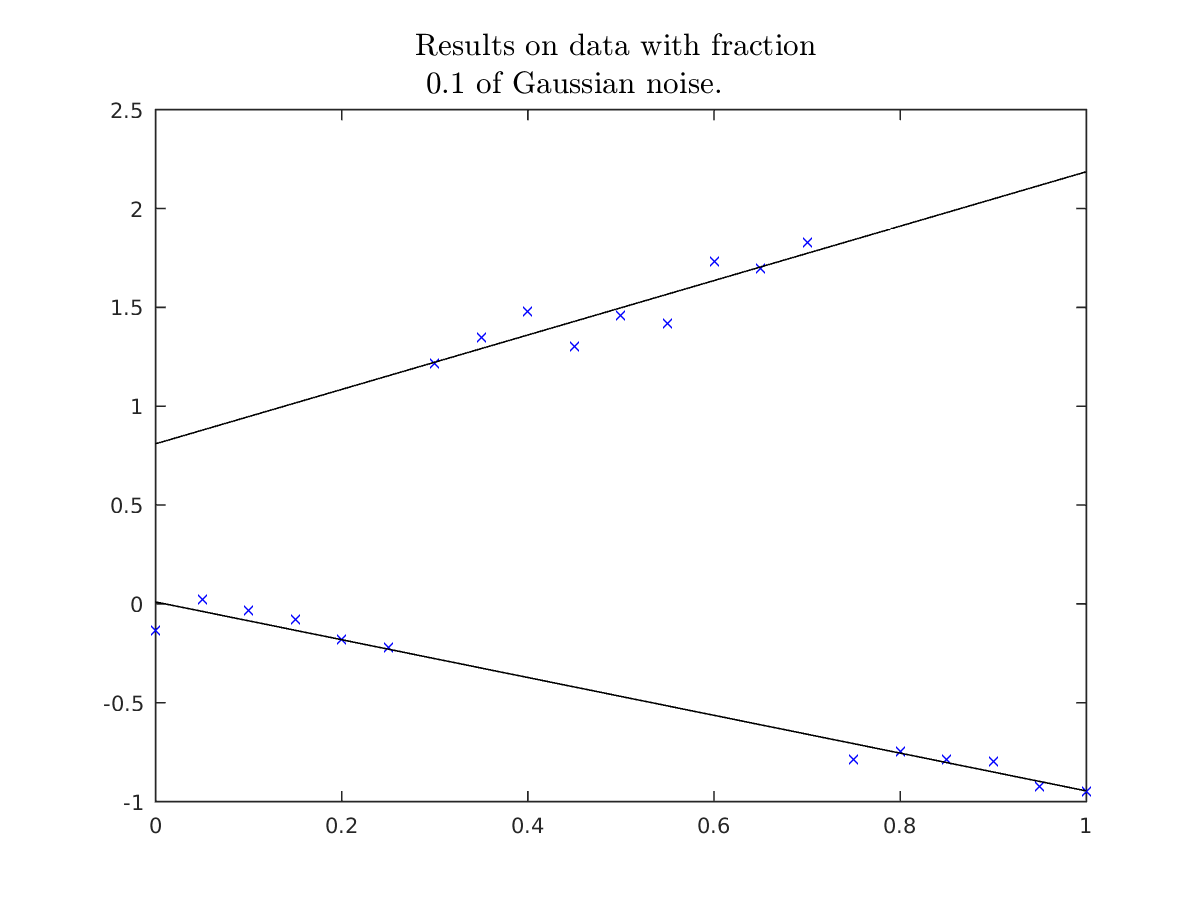
\includegraphics[width= .3\textwidth]{figures/EM_results_noise_1.png} & 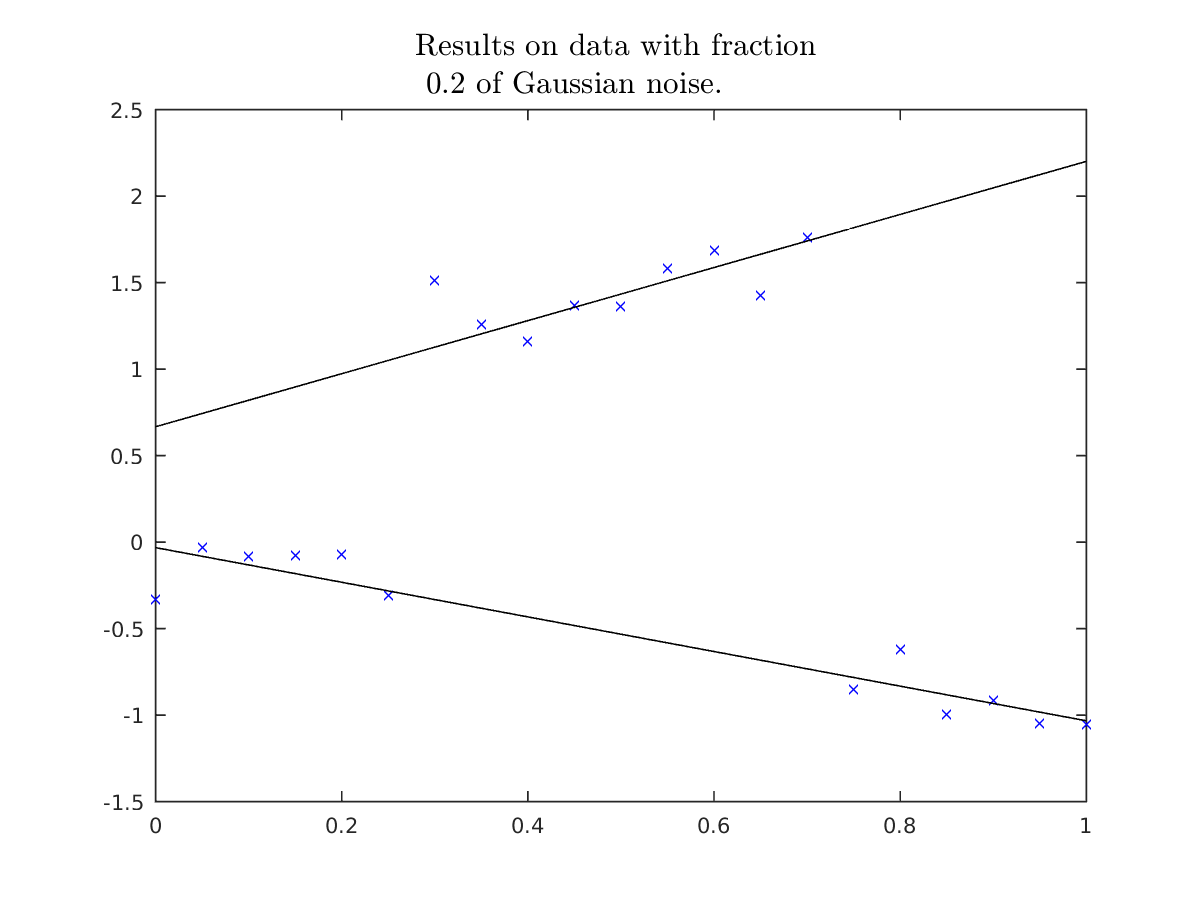
\includegraphics[width= .3\textwidth]{figures/EM_results_noise_2.png}  &
		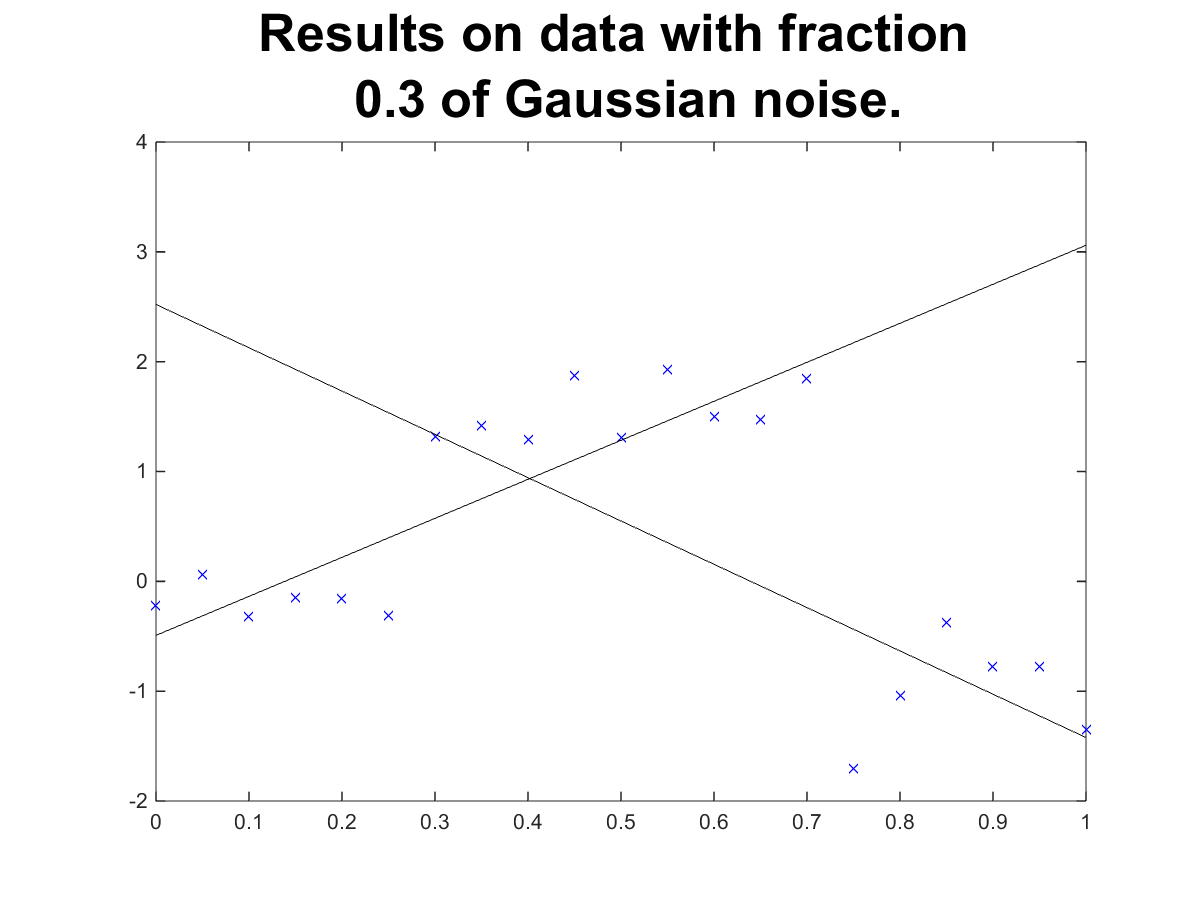
\includegraphics[width= .3\textwidth]{figures/EM_results_noise_3.png} \\ 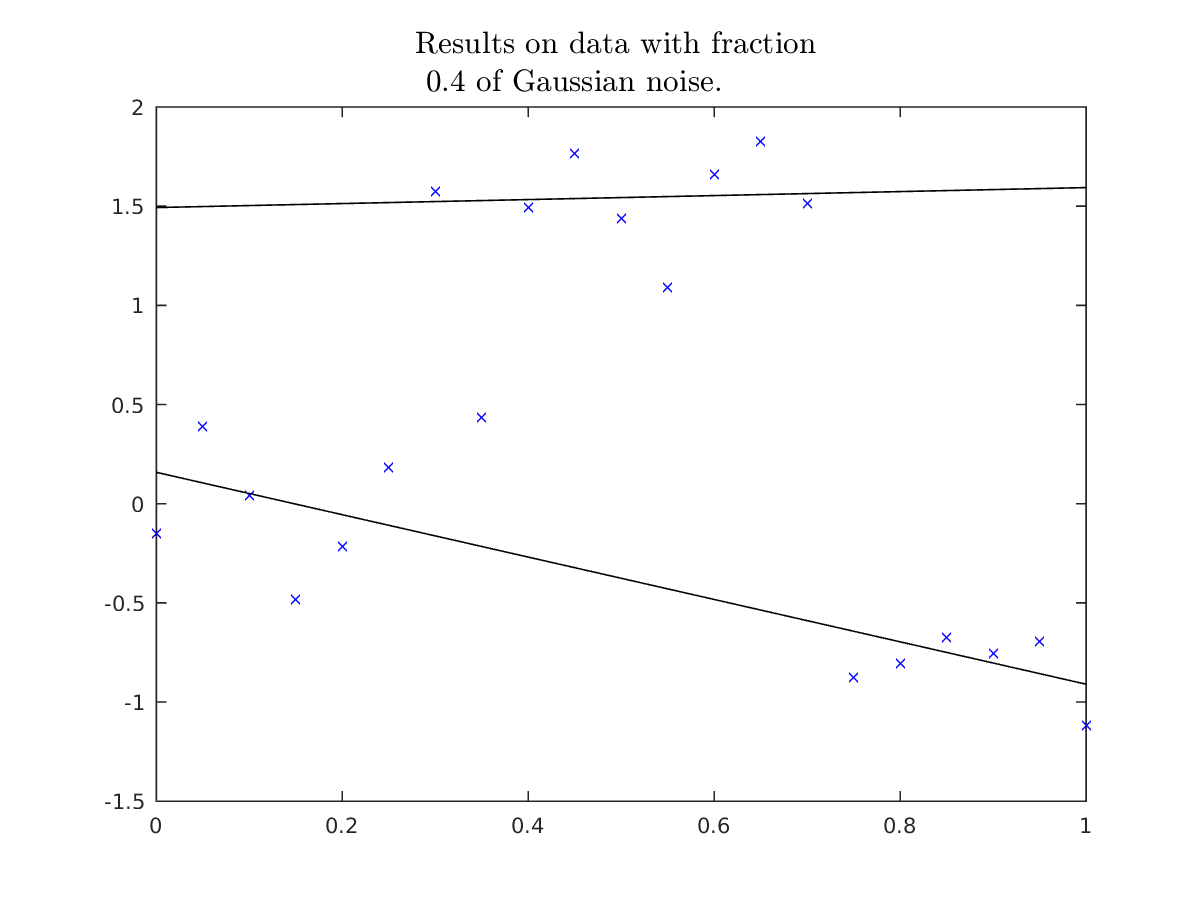
\includegraphics[width= .3\textwidth]{figures/EM_results_noise_4.png} &
		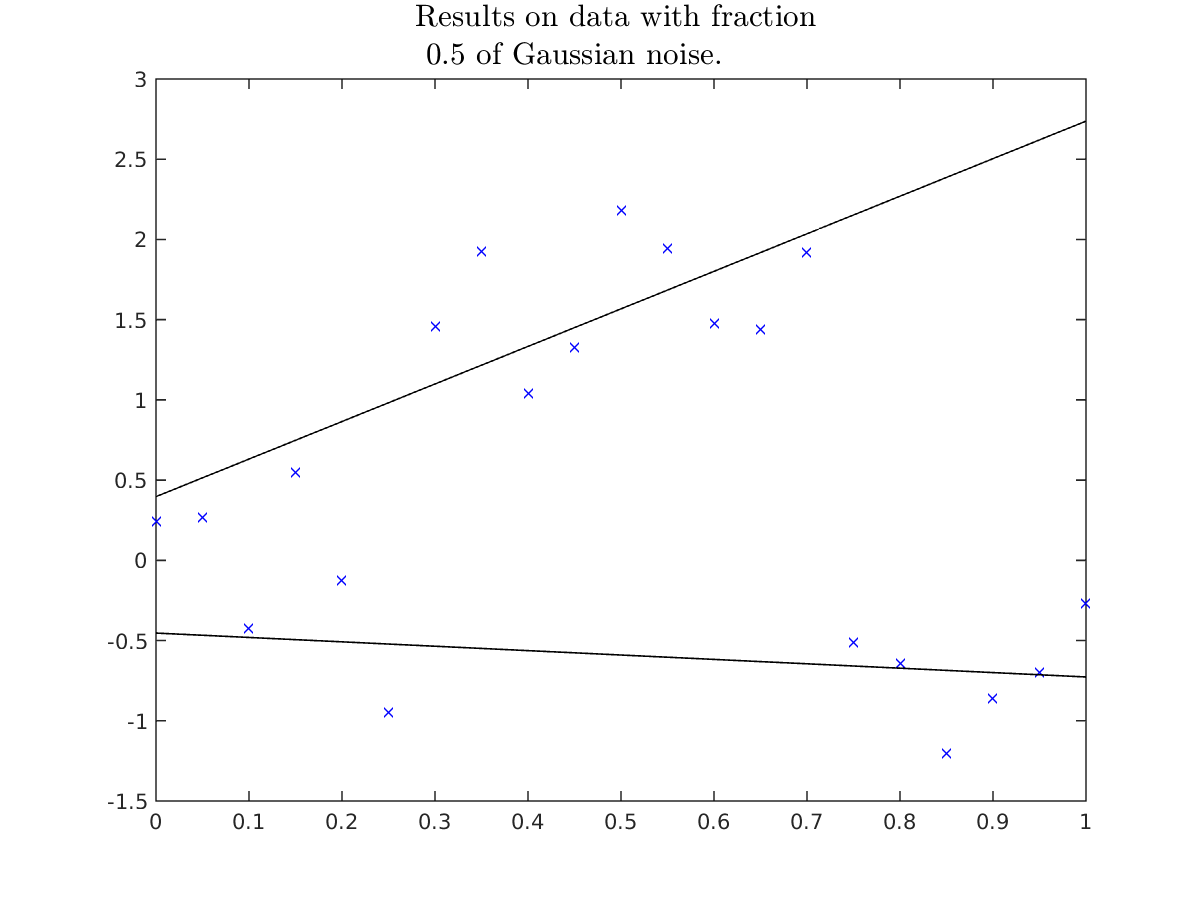
\includegraphics[width= .3\textwidth]{figures/EM_results_noise_5.png} & 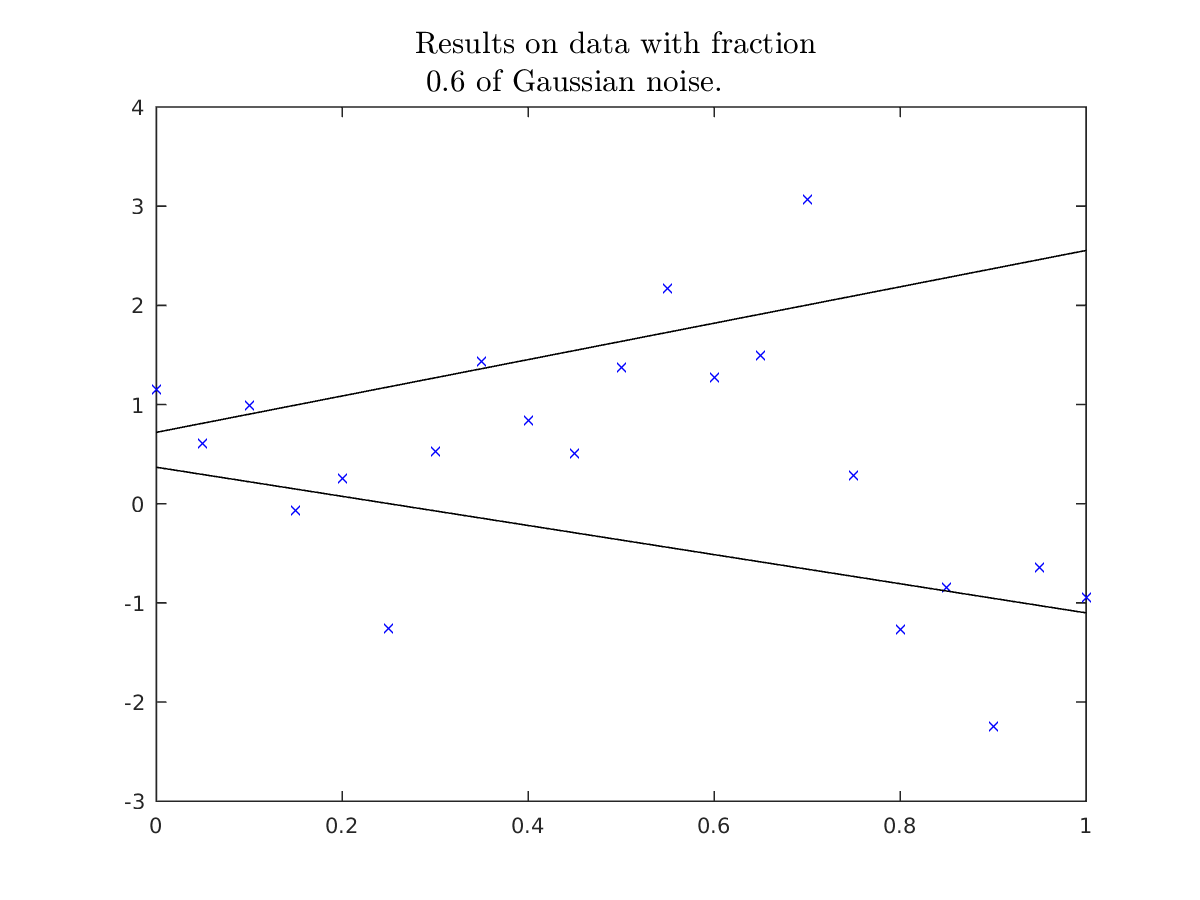
\includegraphics[width= .3\textwidth]{figures/EM_results_noise_6.png} \\
		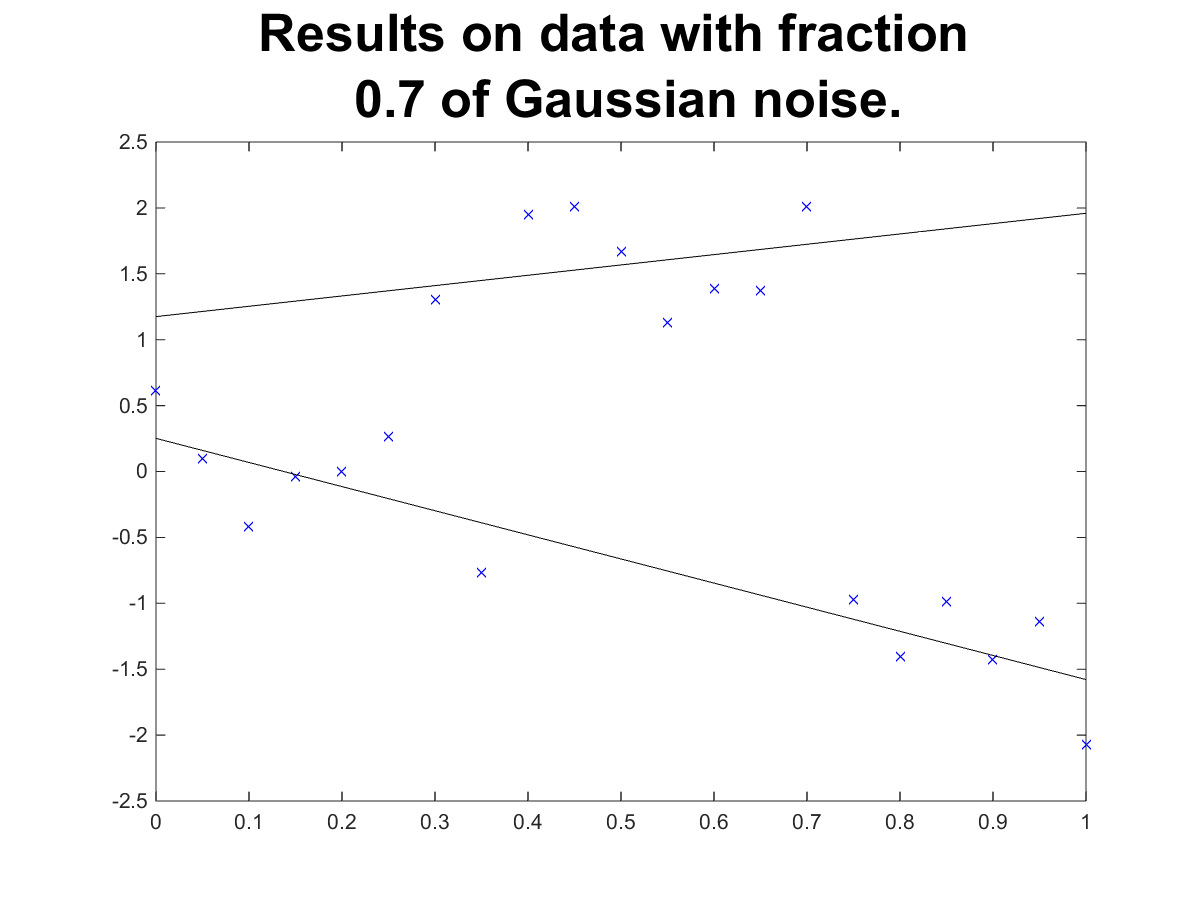
\includegraphics[width= .3\textwidth]{figures/EM_results_noise_7.png} & 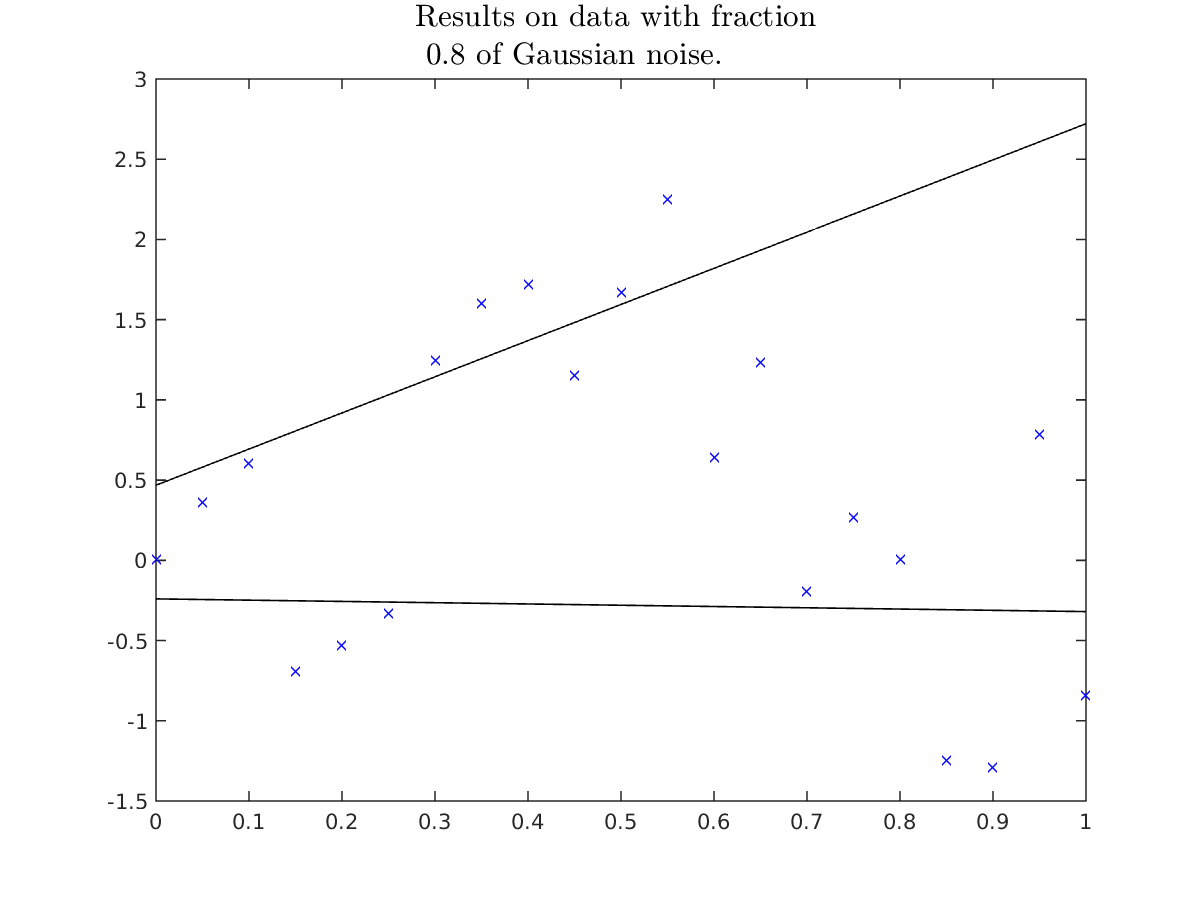
\includegraphics[width= .3\textwidth]{figures/EM_results_noise_8.png} & 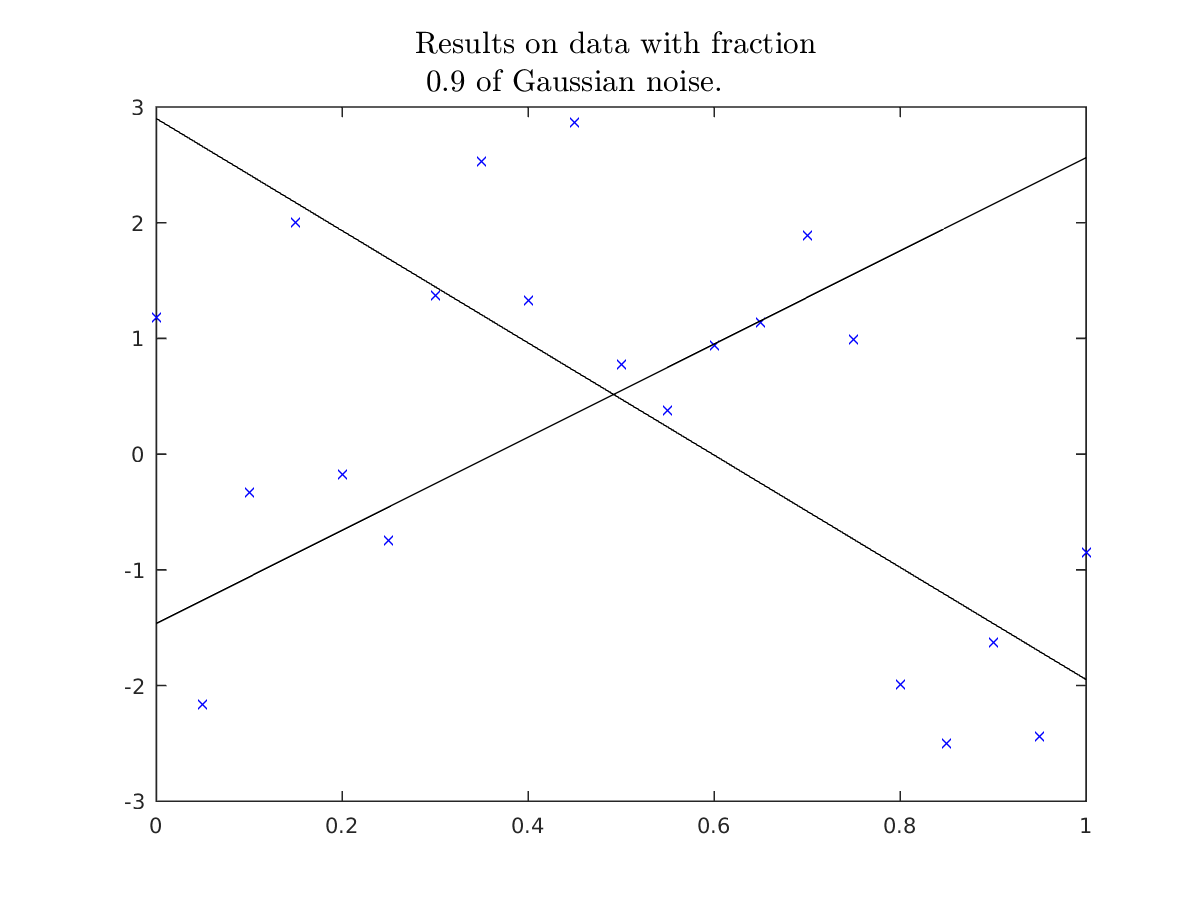
\includegraphics[width= .3\textwidth]{figures/EM_results_noise_9.png}\\ 
		\multicolumn{3}{c}{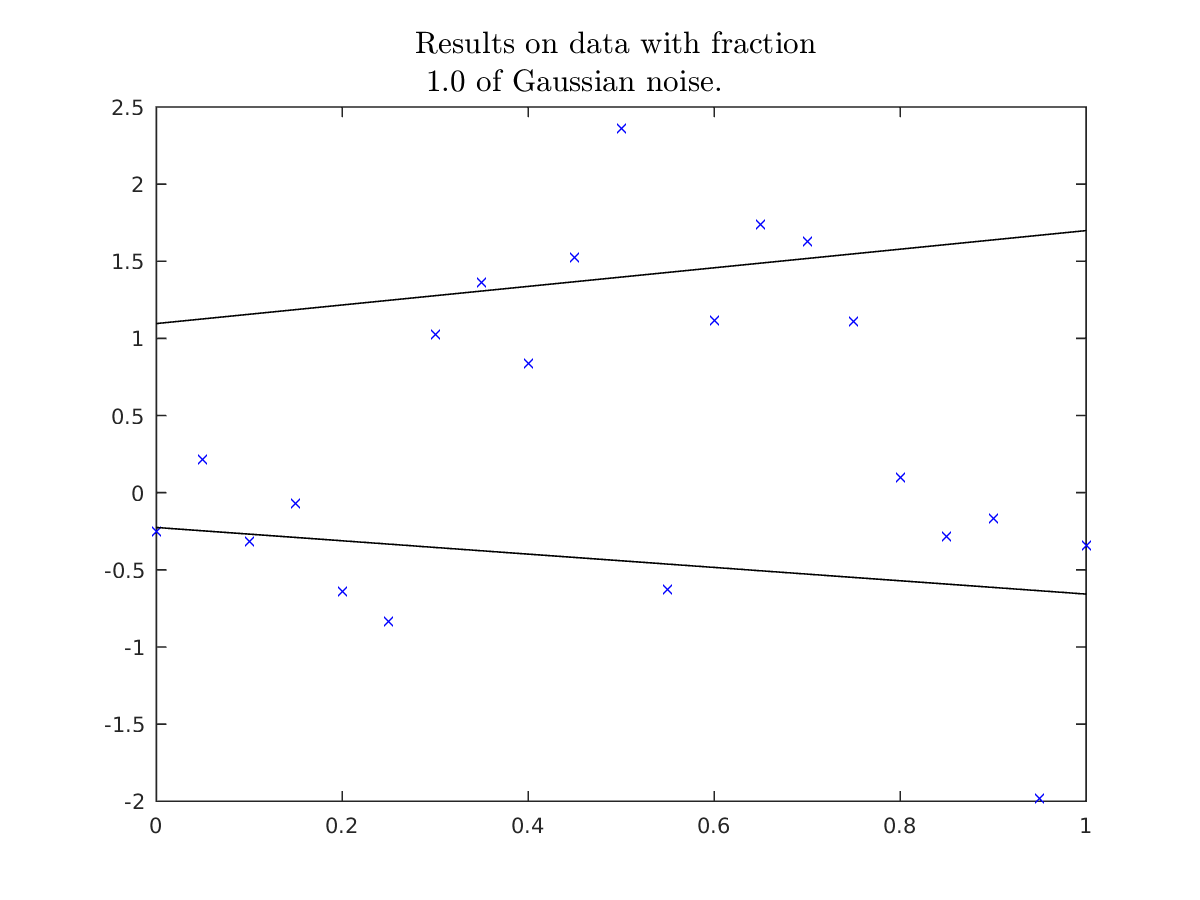
\includegraphics[width= .3\textwidth]{figures/EM_results_noise_10} }
	\end{tabular}
	\caption{Estimating the impact of noise on the result of E-M.}
	\label{fig:Noise-EM}
\end{figure}

Figure \ref{fig:EM-conv} shows the convergence of EM on the dataset from section \ref{sec:pureLineFit} where straightforward line fitting produced a low fidelity result (figure \ref{fig:lineFitting}(c)). Initially, the algorithm begins with a guess on what the lines should be and very quickly (in just two iterations, it seems) converges to a pair of lines which represents the data pretty well. The color-coding on the figures represents the points assigned to the two lines (latent assignment variables $\mathbf{z}$). 

We also experimented with adding noise to the same dataset in order to estimate its impact on the accuracy of the algorithm. We experimented with fractions of Gaussian white noise generated with $\sigma = 1$. Figure \ref{fig:Noise-EM} shows the results. It's not hard to see that a significant amount
of noise causes EM to be unable to converge to a qualitatively acceptable solution.

\section{Mosaicing with RANSAC}

In this section, we outline our approach for dealing with part 2 of the problem set, mosaicing a pair of images with RANSAC.
	
\subsection{SIFT feature extraction}

We first prove that \texttt{VLFeat} is running correctly. Figure \ref{fig:SIFT_feat} visualizes the SIFT features extracted by \texttt{VLFeat}. The \texttt{VLFeat} version used was 0.9.19, and it appears to be extracting denser features than previous versions of the library, perhaps because of less aggressive non-maximum suppression. 

\begin{figure}[H]
	\centering
	\begin{tabular}{ccc}
		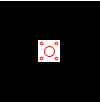
\includegraphics[scale=1.3]{figures/sift_square.png} & 
		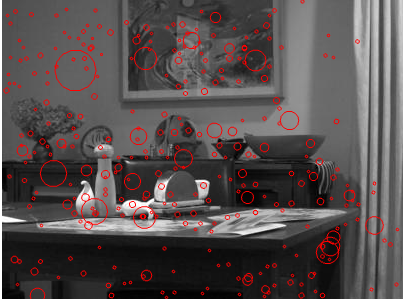
\includegraphics[scale=.4]{figures/sift_left.png} &
		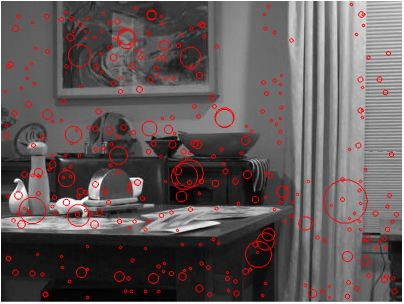
\includegraphics[scale=.4]{figures/sift_right.png} \\ 
		(a) & (b) &(c)
	\end{tabular}
\caption{SIFT feature extraction on a simple intensity square(a) and the provided pictures (b, c).}
\label{fig:SIFT_feat}
\end{figure}

To reproduce these results, run the function \texttt{part2} with parameter 1.

\subsection{Three best matches}

\begin{figure}[H]
	\centering
	\begin{tabular}{cc}
		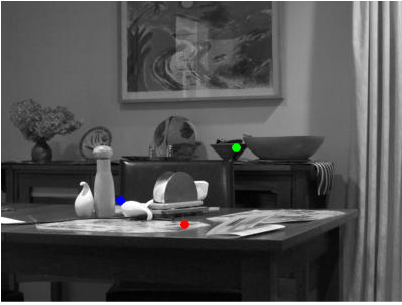
\includegraphics[width=.5\textwidth]{figures/sift_threebest_left}& 
		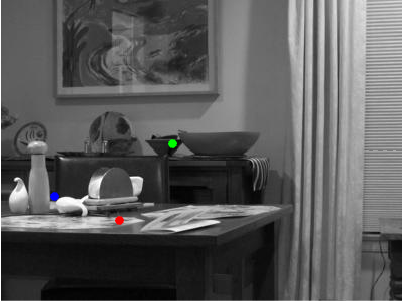
\includegraphics[width=.5\textwidth]{figures/sift_threebest_right} \\
		(a) & (b)
	\end{tabular}
	\caption{Best three matches in terms of Euclidean Distance in SIFT space. Best viewed in color.}
	\label{fig:SIFT_matches}
\end{figure}

Figure \ref{fig:SIFT_matches} contains the color-coded matches between the three best matches that we computed based on SSD between the SIFT histograms. Function \texttt{find\_best\_match.m} implements the matching. To reproduce these results, run the function \texttt{part2} with parameter 2.

\subsection{Affine transformation}

Function \texttt{affine\_transformation.m} uses three 2D point correspondences to solve for the affine transformation that relates them. The output of \texttt{part2(3)} is:

\begin{lstlisting}
>> part2(3)

ans =

1.0e-15 *

   -0.0555    0.1110   -0.2220
   -0.4441   -0.1110   -0.2220
\end{lstlisting}

So the difference between the hard-coded affine transformation and the one found by our MATLAB routine is vanishingly small, and in the order of our system's numerical accuracy about zero.

\subsection{RANSAC}

	Our implementation of RANSAC is contained in MATLAB function \texttt{ransac.m}. In our experiments with the images provided, we ran RANSAC for 1000 iterations. Running \texttt{part2(4)} yields the same matrix for every call, for instance:
	
\begin{lstlisting}

>> part2(4)

A =

   54.6484   69.4537   94.4210
   55.0828   92.7494   90.3263


Ares =

   54.6484   69.4537   94.4210
   55.0828   92.7494   90.3263
\end{lstlisting}

\subsection{Stitching}
\label{sec:stitch}
For this part, we adapted stitching code available online \footnote{\href{http://tobw.net/index.php?cat_id=2&project=Panorama+Stitching+Demo+in+Matlab}{Panorama Stitching in MATLAB.}} to our needs. The function \texttt{stitch.m} calculates both a stitched image as well as the enveloping mask, such that future stitchings of the resulting images can be made possible (an already existing mask is among the optional arguments to the method). The method uses the MATLAB built-ins \texttt{maketform} and \texttt{imtransform} instead of the recommended \texttt{affine2d} and \texttt{imwarp} since it needs to make use of the second and third return values of \texttt{imtransform} (\texttt{XData} and \texttt{YData}, respectively) to calculate the position of the transformed images in the common co-ordinate system of both images.

The entire code is available in \texttt{stitch.m}. Figure \ref{fig:stitched_static} contains the results of calling \texttt{part2(5)}, which stitches the original ``left" part of the dining room image (LR1bw) and two affine transformations which we also had to implement (\texttt{translate100} and \texttt{trs}).

\begin{figure}[H]
	\centering
	\begin{tabular}{ccc}
		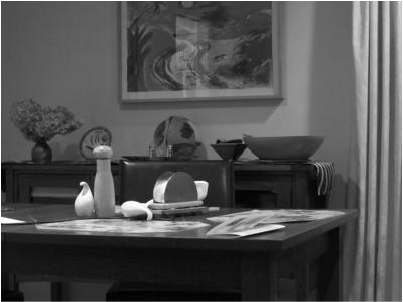
\includegraphics[scale=.4]{LR1bw.png} &
		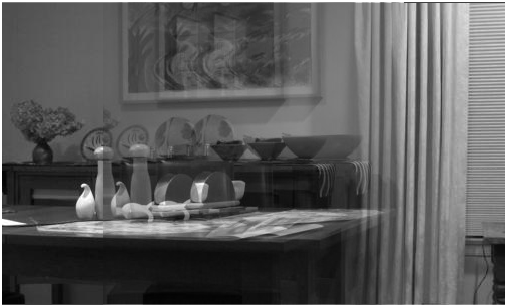
\includegraphics[scale=.4]{figures/tr100stitching} &
		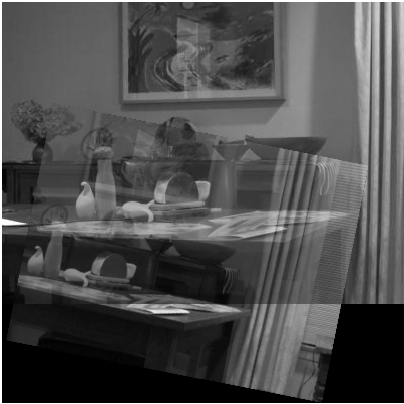
\includegraphics[scale=.4]{figures/tr_rot_sc_stitching} \\	
		(a) & (b) & (c)
	\end{tabular} 
	\caption{The result of stitching between (a) the original image, (b) Its translation at x = +100 and (c) A rotation by $\pi$/16, scaling by 0.8, and a translation of (50, 100). Note that the results are not aesthetically pleasing because the transformations in this section of the problem set have not been computed by RANSAC, but are statically provided to the stitching algorithm.}
	\label{fig:stitched_static}
\end{figure}

\subsection{Mosaicing}

Calling \texttt{part2(6)} performs our full image mosaicing algorithm. The result can be found in figure \ref{fig:mosaic}.
We can see that the transformation recovered by RANSAC is a translation almost entirely along the x axis. 

\begin{figure}[H]
	\centering
	\begin{tabular}{ccc}
		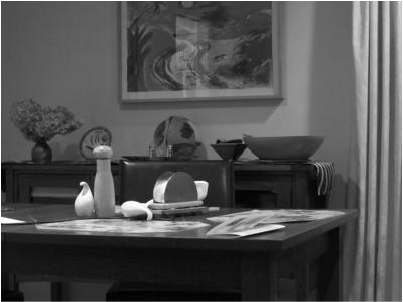
\includegraphics[scale=.4]{LR1bw} &
		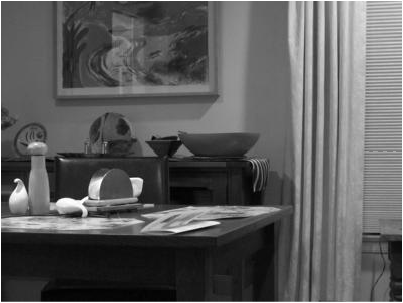
\includegraphics[scale=.4]{LR2bw} & 
		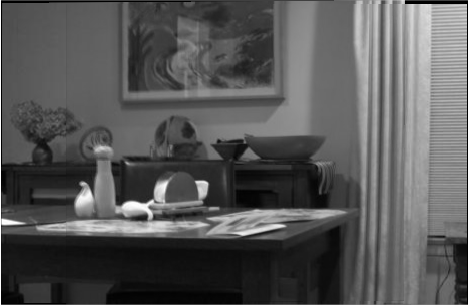
\includegraphics[scale=.4]{figures/mosaic1} \\
		(a) & (b) & (c)		
	\end{tabular}	
	\caption{Mosaicing images (a) and (b) yields (c).}
	\label{fig:mosaic}
\end{figure}

\subsection{Results on custom images}

In this section, we perform mosaicing on custom images. Our results can be reproduced by running \texttt{part2(7)}.

\subsubsection{Dining room images}

The first image pair that we test on consists of the left part of the original dining room image, as well as its transformation induced by \texttt{trs}, which was already used in section \ref{sec:stitch}. That is, we applied the transformation to the original image (using \texttt{affine2d} and \texttt{imwarp}), saved the resulting image under the subdirectory ``figures", and then loaded both images to perform mosaicing on them. Figure \ref{fig:mosaicPair1} contains the results. It is evident that the results are quite aesthetically pleasing, up to some intensity blurring.

\begin{figure}[H]
	\centering
	\begin{tabular}{ccc}
		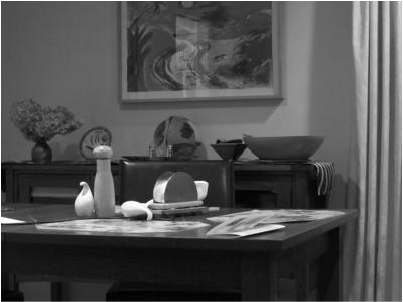
\includegraphics[width=.3\textwidth]{LR1bw} & 
		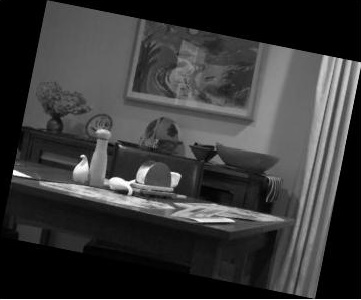
\includegraphics[width=.3\textwidth]{figures/rotated_figure} & 
		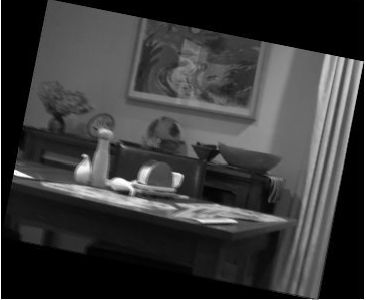
\includegraphics[width=.3\textwidth]{figures/mosaic_rotation} \\
		(a) & (b) & (c)
	\end{tabular}
	\caption{Mosaicing images (a) and (b) yields (c).}
	\label{fig:mosaicPair1}
\end{figure}

\subsubsection{Our room}

We also took a pair of pictures from a wall in our room in College Park. Figure \ref{fig:roomImgOrig} shows the original image in B \& W. We divide this image into two portions which are overlapping by approximately 70\% and then mosaic them. The results are shown in figure \ref{fig:mosaicPair2} and are quite pleasing, but for a small vertical white line approximately a third of the way from the left. 

\begin{figure}[H]
	\centering
	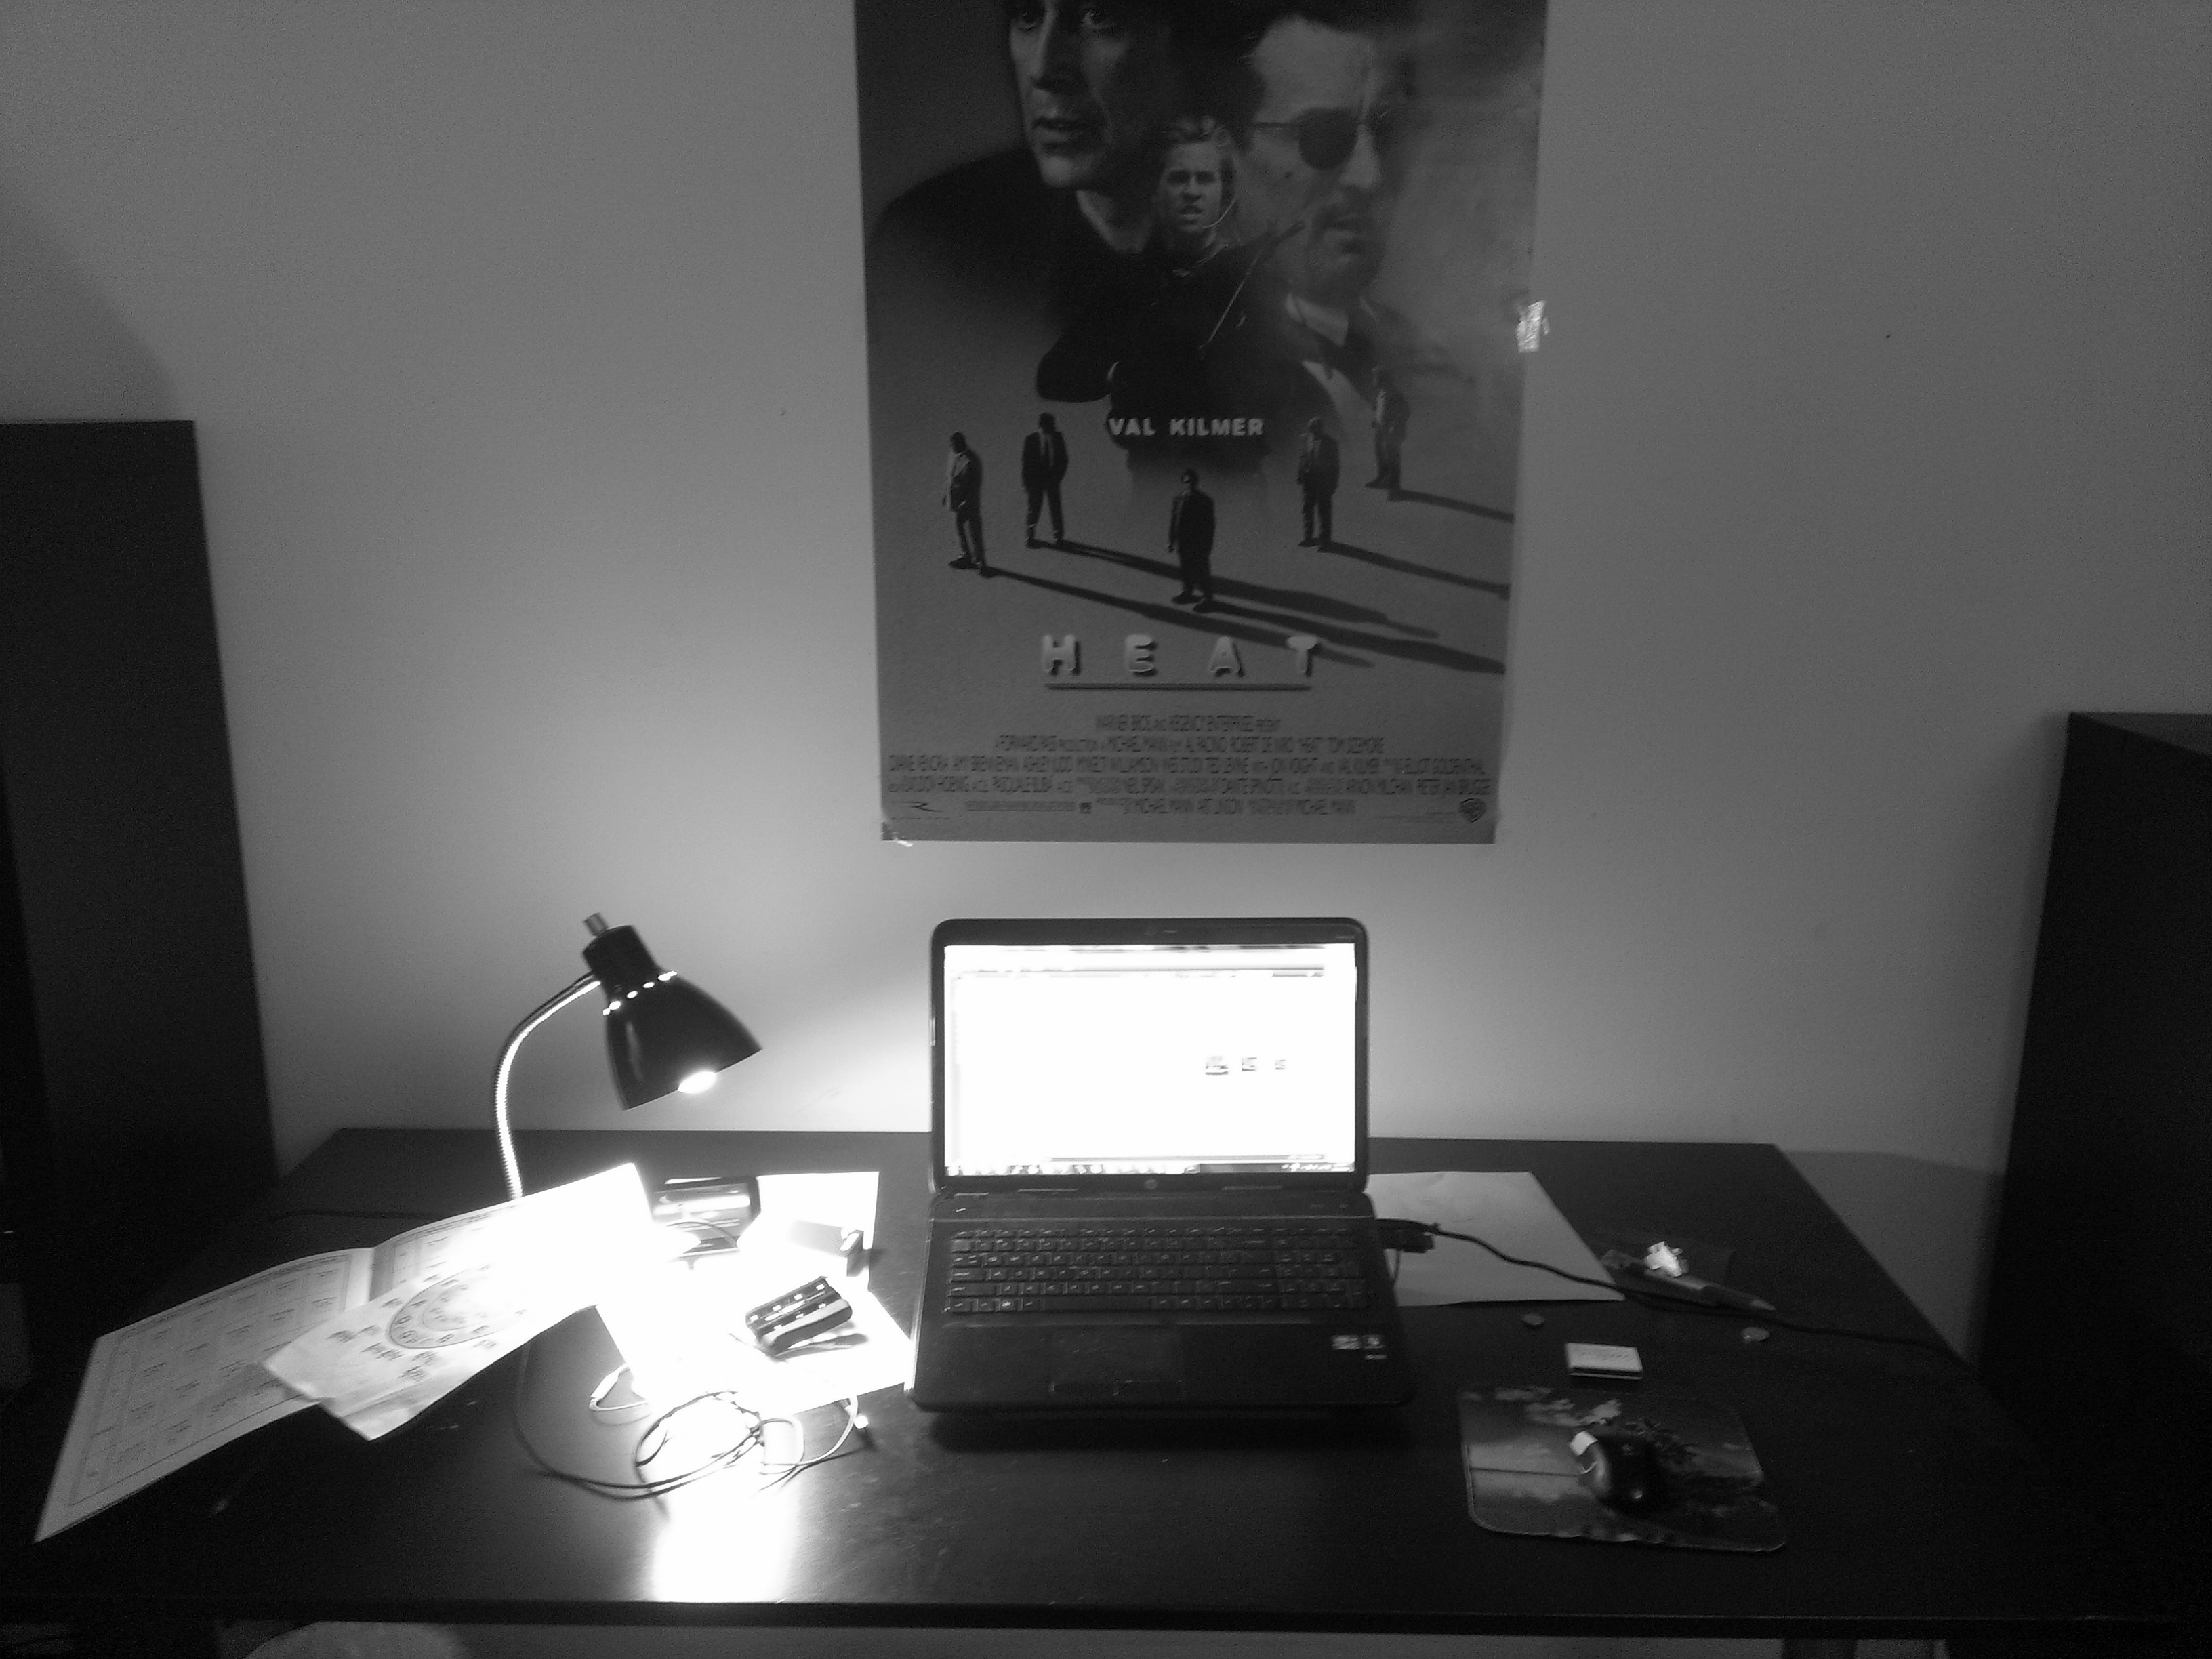
\includegraphics[scale=.065]{figures/room_b_w}
	\caption{A picture of our bedroom wall.}
	\label{fig:roomImgOrig}
\end{figure}

\begin{figure}[H]
\centering
	\begin{tabular}{ccc}
			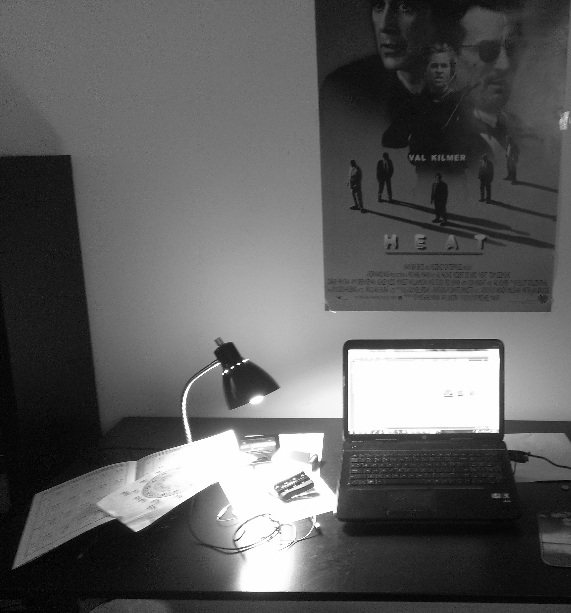
\includegraphics[scale=.20]{figures/room_l} & 
			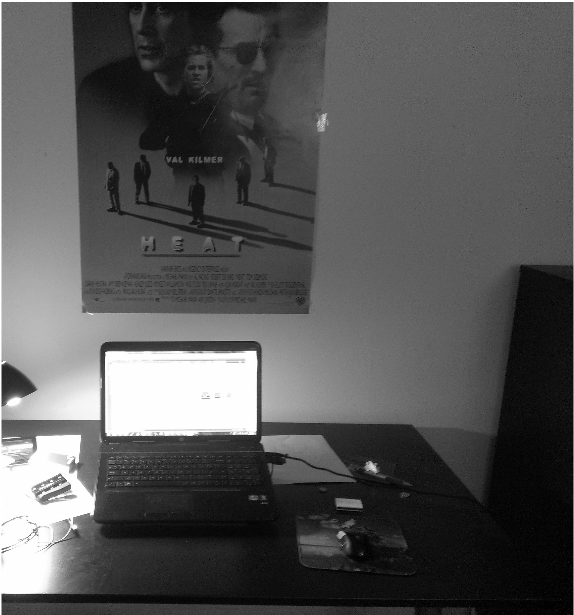
\includegraphics[scale=.20]{figures/room_r} &
			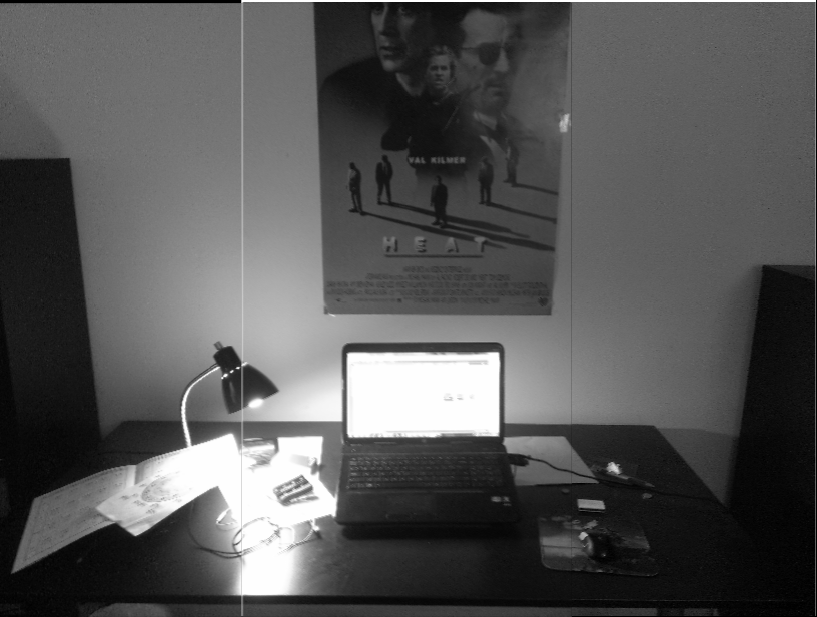
\includegraphics[scale=.20]{figures/room_mosaic} \\ 
		(a) & (b) & (c)
	\end{tabular}
	\caption{Mosaicing images (a) and (b) yields (c).}
	\label{fig:mosaicPair2}
\end{figure}

We also experiment by applying the transformation \texttt{trs} to the image in figure \ref{fig:mosaicPair2}(a) and mosaicing the two images. The results can be viewed in figure \ref{fig:mosaic2Pair2} and are also of high fidelity.

\begin{figure}[H]
\centering
	\begin{tabular}{ccc}
			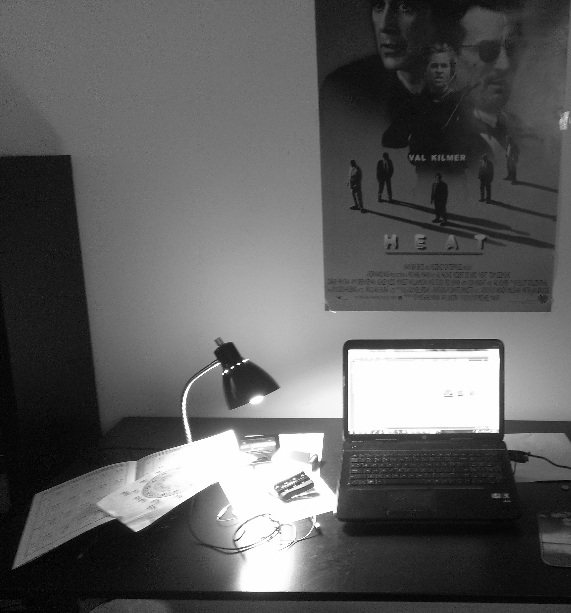
\includegraphics[scale=.25]{figures/room_l} & 
			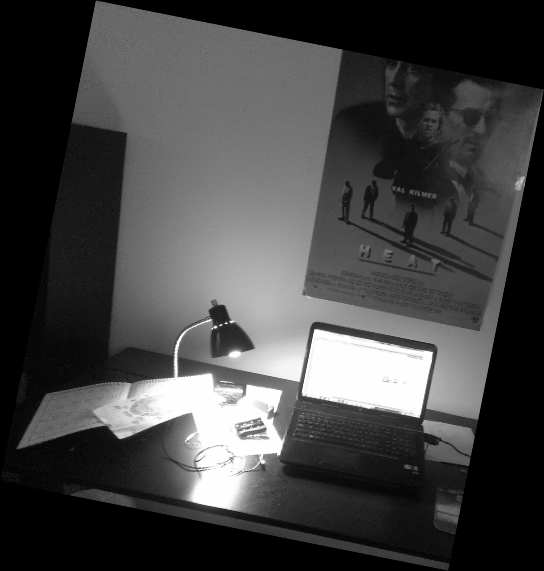
\includegraphics[scale=.25]{figures/room_trs} &
			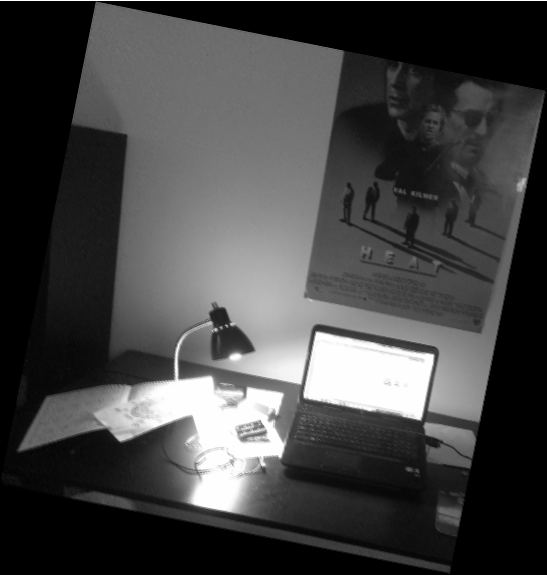
\includegraphics[scale=.25]{figures/room_mosaic2} \\ 
		(a) & (b) & (c)
	\end{tabular}
	\caption{Mosaicing images (a) and (b) yields (c).}
	\label{fig:mosaic2Pair2}
\end{figure}
\end{document}